\section{Из чего состоит компьютер}\label{base:introduction:components}
\subsection{Общий обзор}\label{base:introduction:components:review}
Рассмотрим типичный персональный компьютер. В общем случае он состоит из устройства вывода изображения (монитор), большой шумящей коробки (системный блок) и разных устройств поменьше.
\begin{figure}[h!]
 \centering
 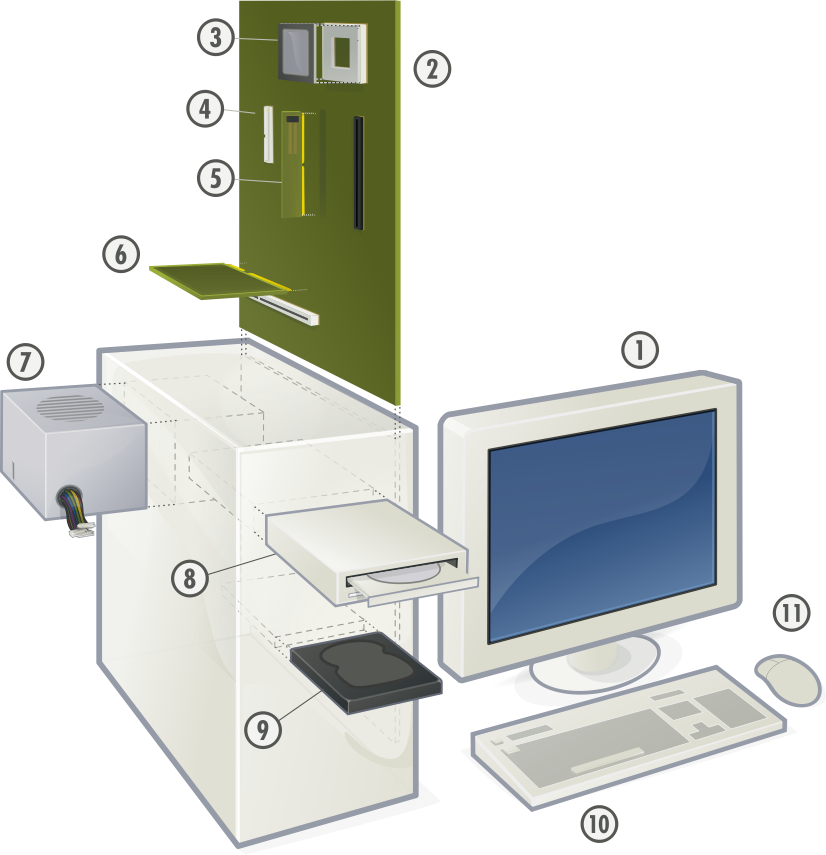
\includegraphics[width=0.5\textwidth]{base/Introduction/Computer.png}
 \label{Base:introduction:components:review:computerpic}
 \caption{Устройство персонального компьютера:}
 \footnotesize
 \begin{enumerate}
  \item монитор;
  \item материнская плата;
  \item процессор;
  \item порт ATA;
  \item оперативная память;
  \item карты расширений;
  \item блок питания;
  \item дисковод;
  \item жёсткий диск;
  \item клавиатура;
  \item компьютерная мышь;
 \end{enumerate}
\end{figure}

\subsection{Системный блок}\label{base:introduction:components:case}
Начнём наше знакомство с основного компонента настольного компьютера --- \emph{системного блока} (англ.~\emph{computer case} или \emph{computer chassis}). Сам по себе системный блок (по какой-то совершенно неясной причине иногда называемый <<процессором>>; наука пытается найти объяснение этому явлению) является корпусом, в котором располагаются все основные компоненты.
\begin{figure}[h!]
 \centering
 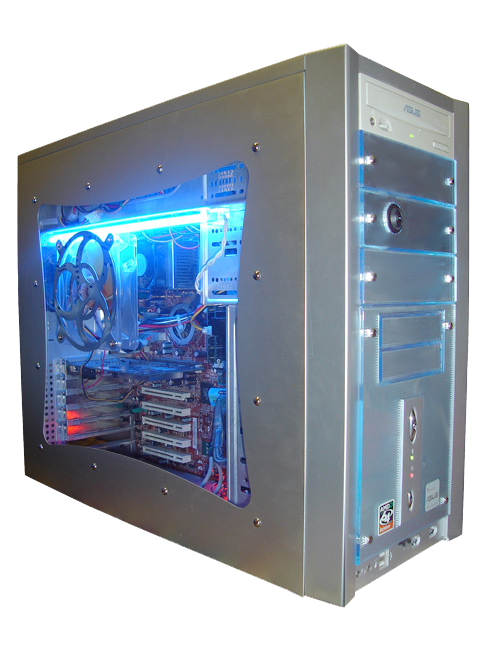
\includegraphics[width=0.5\textwidth]{base/Introduction/Case.png}
 \caption{Типичный системный блок}
 \label{base:introduction:components:case:typicalcasepic}
\end{figure}
\begin{figure}[h!]
 \centering
 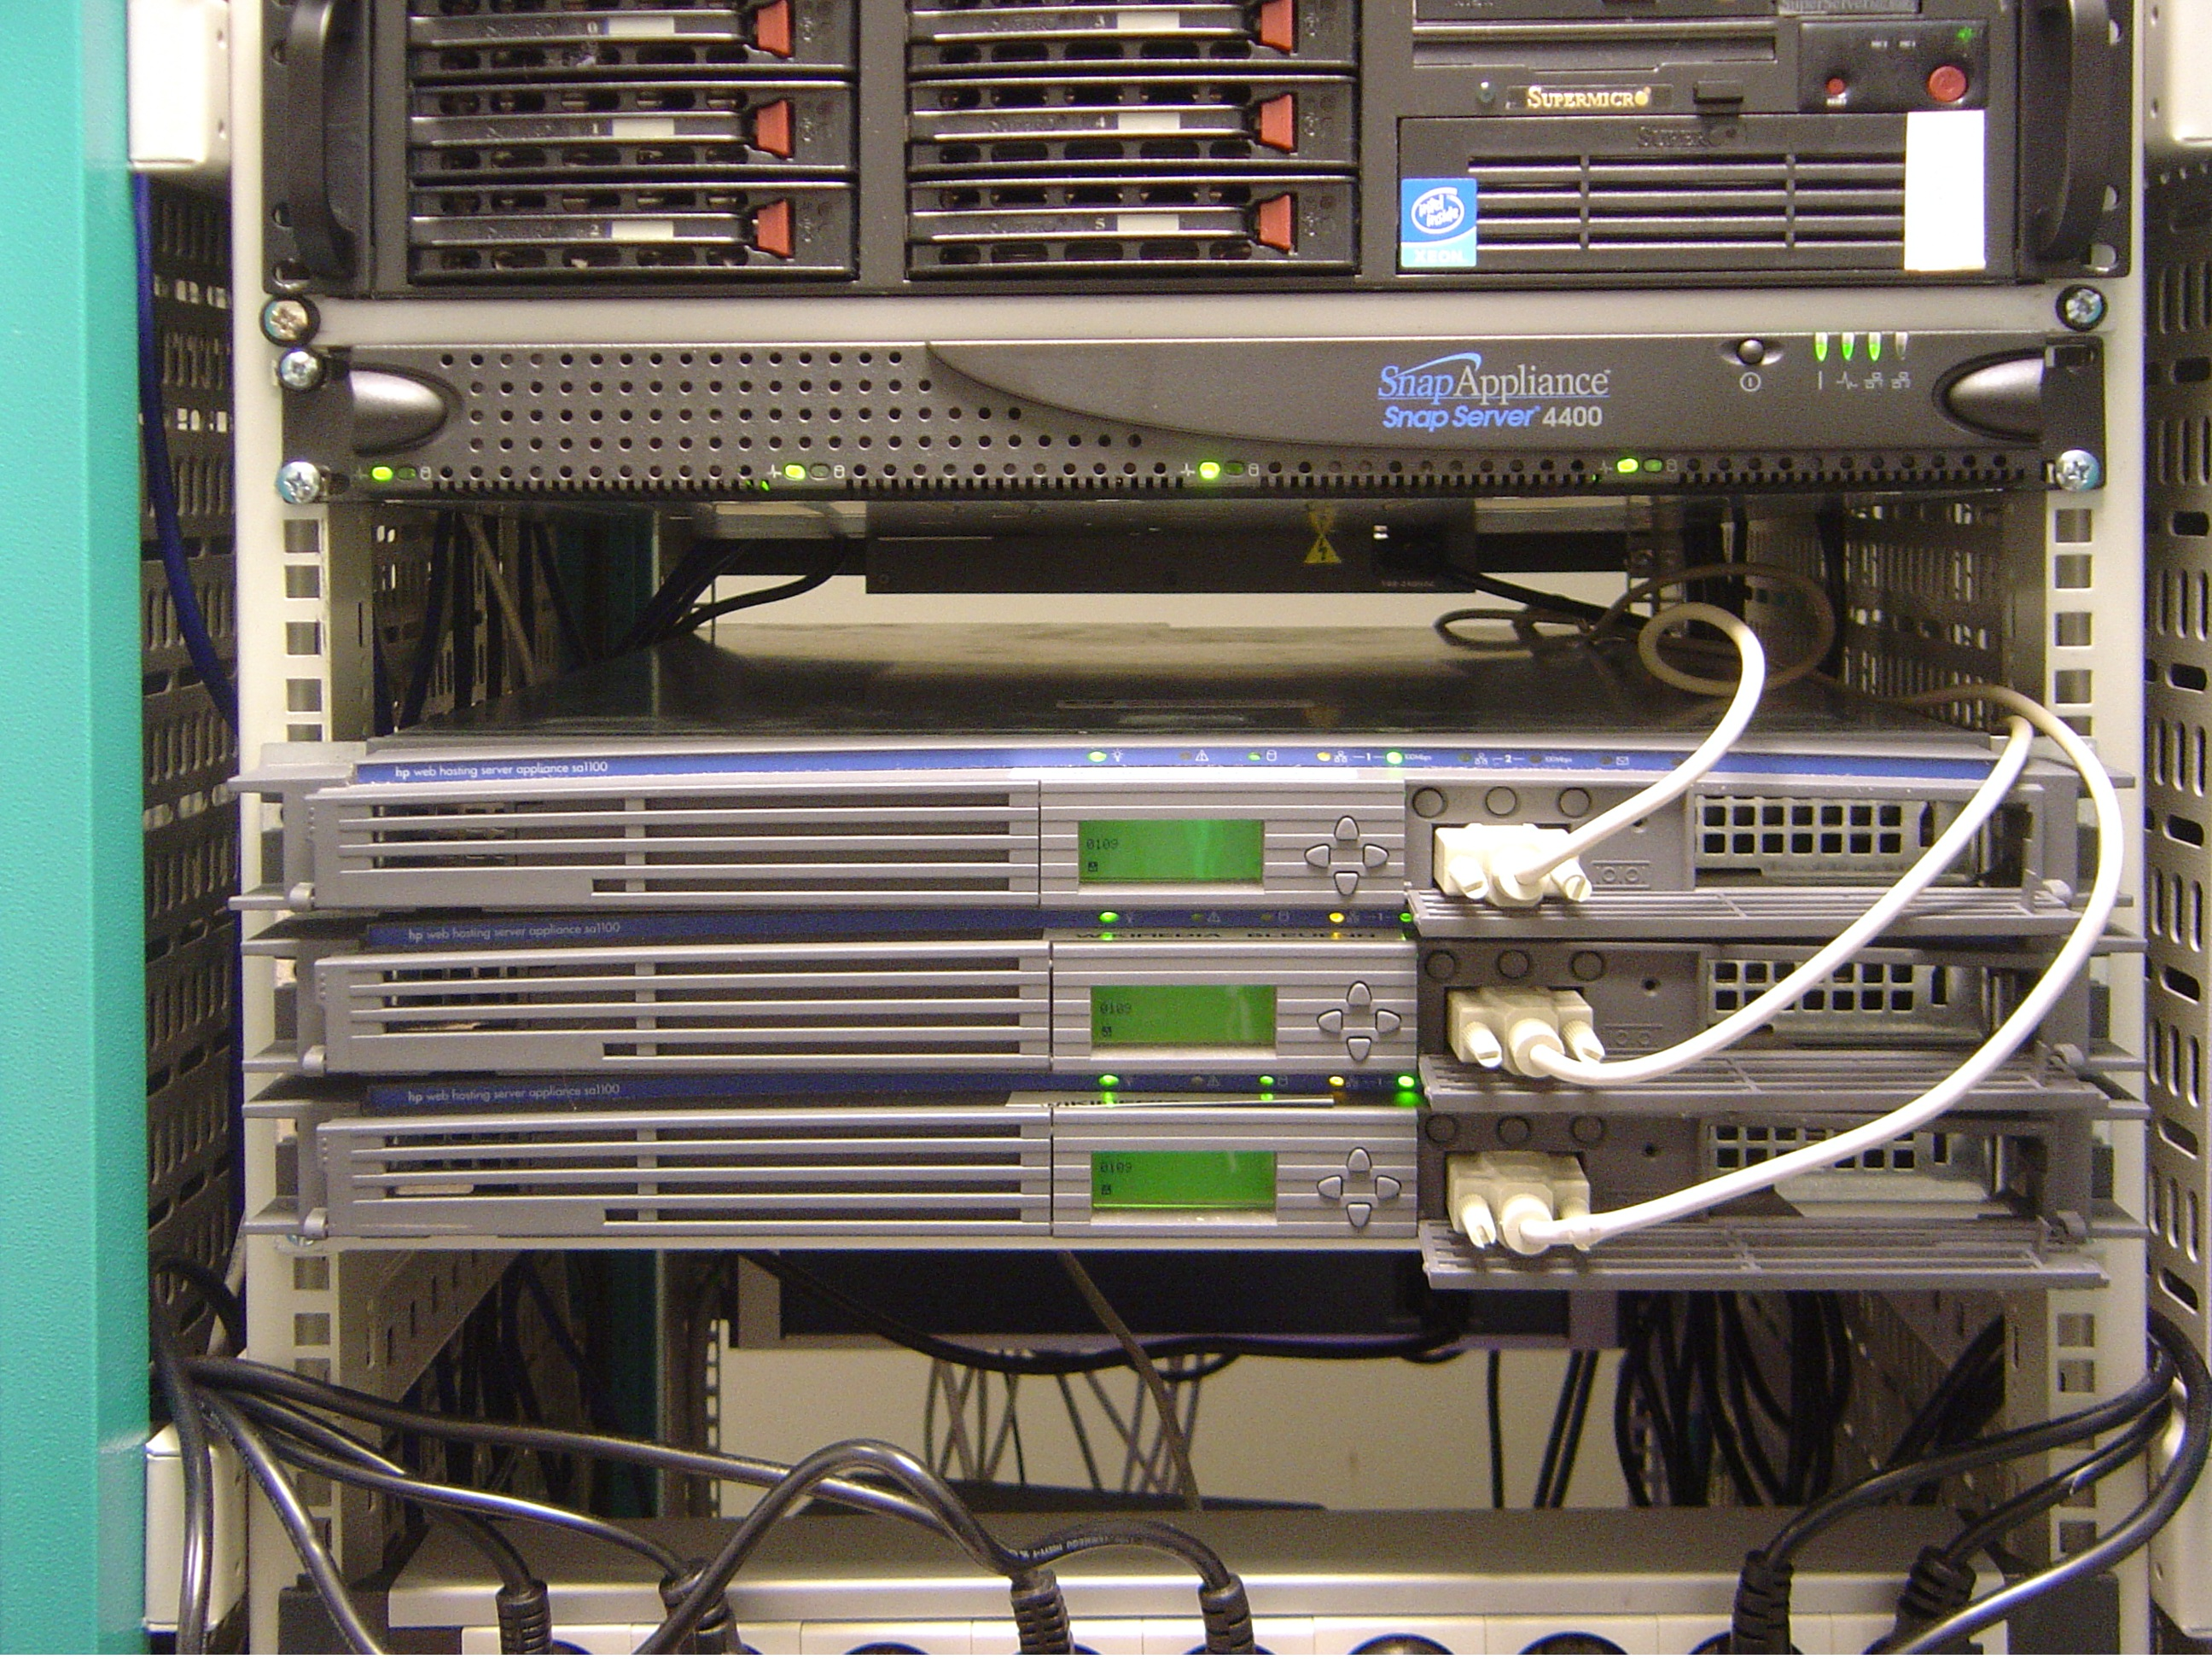
\includegraphics[width=0.5\textwidth]{base/Introduction/Case_wikipedia.jpg}
 \caption{Корпуса серверов Википедии}
 \label{base:introduction:components:case:wikipediacasepic}
\end{figure}
Внутреннее пространство поделено на несколько секций: отсек под устройства формата 5,25 дюймов, отсек под устройства формата 3,5 дюйма, место крепления блока питания и место для крепления материнской платы.

Корпуса могут быть разных форм и размеров. Относительно пропорций есть два устоявшихся форм-фактора: горизонтальные и вертикальные. Среди горизонтальных форм-факторов можно отметить:
\begin{description}
 \item[Desktop] $533\times419\times152$\,мм
 \item[FootPrint] $406\times406\times152$\,мм
 \item[SlimLine] $406\times406\times101$\,мм
 \item[UltraSlimLine] $381\times352\times75$\,мм
\end{description}
Также к горизонтальным форм-факторам можно причислить стоечные корпуса.

Вертикальные форм-факторы встречаются наиболее часто в офисах, домах, компьютерных классах. Они объеденены общим названием \emph{Tower} (minitower, miditower, bigtower). Среди причин их распространённости можно отметить больший размер по сравнению с горизонтальными, за счёт чего внутри остаётся больше места для вентиляции или дополнительных компонентов.

Вне зависимости от форм-фактора, системный блок является своеобразной <<печкой>>. Для охлаждения устройств, расположенных в нём, используется система вентиляции или циркуляции охлаждённой жидкости. Вентиляцию обеспечивают специальные вентиляторы (\emph{кулеры}, англ. \emph{cooler}), расположенные как на наиболее тепловыделяющих уст\-ройствах, так и на самом корпусе.
Довольно часто кулеры ставятся парно и однонаправлено, таким образом получается, что один задумает воздух внутрь, а другой выдувает наружу. За счёт этого обеспечивается постоянный поток воздуха, который оказывает охлаждающее действие.
Также кулеры устанавливают на одну из боковых стенок вертикальных форм-факторов, и иногда на вертикальные. Т.\,к.~охлаждение --- необходимый для нормального функционирования компьютера процесс, к его осуществлению надо подходить очень внимательно.
В частности, представляется недопустимым помещение системных блоков в тестные ниши современных компьютерных столов, т.\,к.~ограниченность пространства этих ниш делает задачу охлаждения труднорешаемой, а установленные средства воздушного охлаждения --- малоэффективными.

\subsubsection{Центральный процессор}\label{base:introduction:componenents:cpu}
\subsubsection{Арифметическо-логическое устройство}\label{base:introduction:components:alu}
\subsubsection{Оперативная память}\label{base:introduction:components:ram}
\begin{figure}[h!]
 \centering
 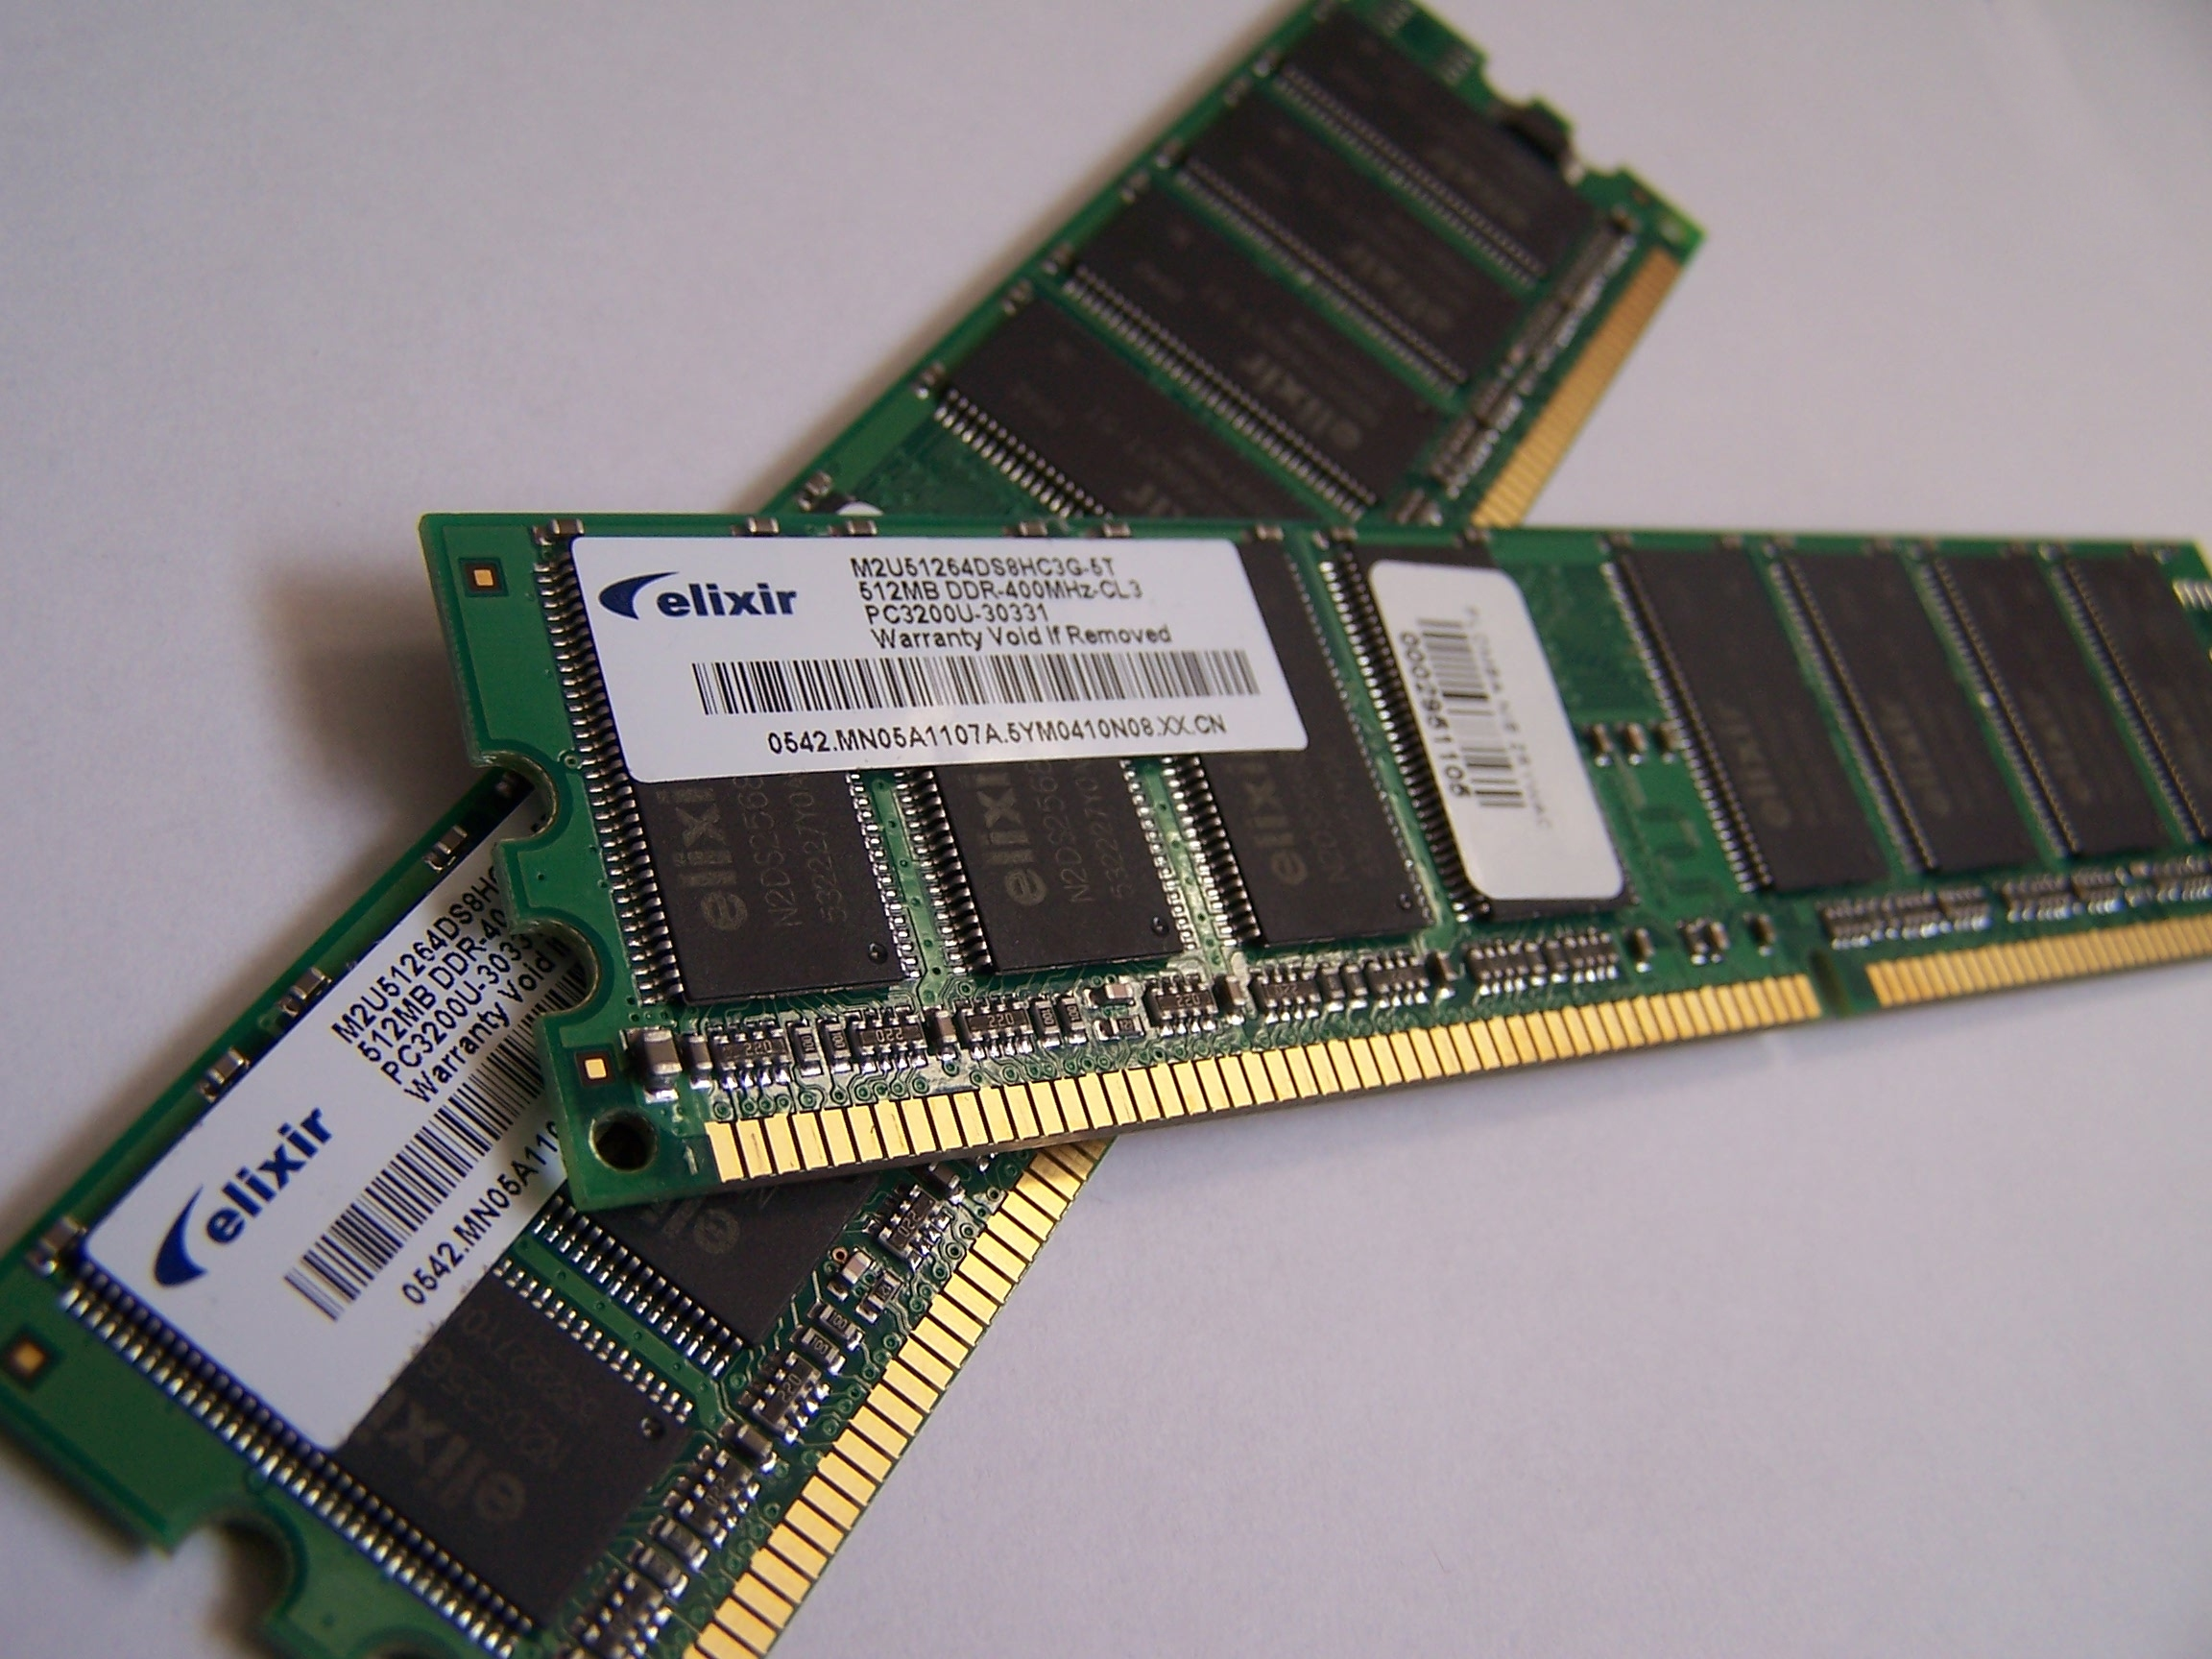
\includegraphics[width=0.5\textwidth]{base/Introduction/Memory.jpg}
 \label{base:introduction:components:ram:rampic}
 \caption{Плашки памяти DDRAM}
\end{figure}
\subsubsection{Материнская плата}\label{base:introduction:components:motherboard}
\subsubsection{Видеокарта}\label{base:introduction:components:videocard}
\subsubsection{Звуковая карта}\label{base:introduction:components:soundcard}
\subsubsection{Сетевая карта}\label{base:introduction:components:nic}
\subsubsection{Блок питания}\label{base:introduction:components:psu}
\subsection{Монитор}\label{base:introduction:components:monitor}
\subsection{Периферия}\label{base:introduction:components:peripheral}
\subsection{Принтеры, сканеры и МФУ}\label{base:introduction:components:printers}
